
\documentclass{article}

%encoding
%--------------------------------------
\usepackage[utf8]{inputenc}
\usepackage[T1]{fontenc}
%--------------------------------------

\usepackage{geometry}
\usepackage{amsmath}
\usepackage{graphicx}
\usepackage{float}

\usepackage[brazilian]{babel}
\usepackage{hyphenat}
\hyphenation{mate-mática recu-perar}

 \geometry{
 a4paper,
 total={170mm,257mm},
 left=20mm,
 top=20mm,
 }

\title{Relatório do trabalho 3}
\date{22/05/2019}
\author{Allan Nozomu Fukasawa RA:163527}

\begin{document}
\maketitle

\section{Introdução}

O objetivo deste trabalho é aplicar operadores morfológicos para segmentar regiões compreeendendo \textit{texto} e \textit{não texto} em uma imagem, utilizando algumas métricas e razões para sua classificação. Além disso, utilziando operadores morfológicos, segmentar cada componente compreeendendo \textit{texto} em palavras.

Os passos seguidos para a execução do trabalho foram extraídos de sua especificação. \cite{Helio:1}

\section{Componentes}

Está sendo enviado junto a este relatório os seguintes arquivos e diretórios:

\begin{itemize}
  \item arquivo Trabalho 3.ipynb: contém todo o código executado durante este trabalho.

  \item três imagens utilizadas durante o processamento: uma (\textit{bitmap.pbm})disponibilizada pelo professor e que foi usada durante o desenvolvimento e as outras duas (\textit{bitmap2.pbm} e \textit{bitmap3.pbm}) para se fazer testes e verificar se os resultados estão condizentes.

  \item diretório res: dentro do diretório \textit{res} contém mais diretórios com os nomes das imagens utilizadas durante o desenvolvimento, sendo um para cada imagem. Dentro de cada diretório da imagem existem todos os componentes conexos detectados, imagens obtidas durante o processamento e a classificação em dois diretórios (\textit{texts} e \textit{not\_texts}) dos componentes.
  
  \item imagens auxiliares em formato .png: para compor o relatório e mostrar os resultados obtidos
  
\end{itemize}

A imagem padrão que está sendo utilizada no programa e também nos resultados apresentados neste relatório é a imagem \ref{Fig:original}

\begin{figure}[!htb]
  \centering
  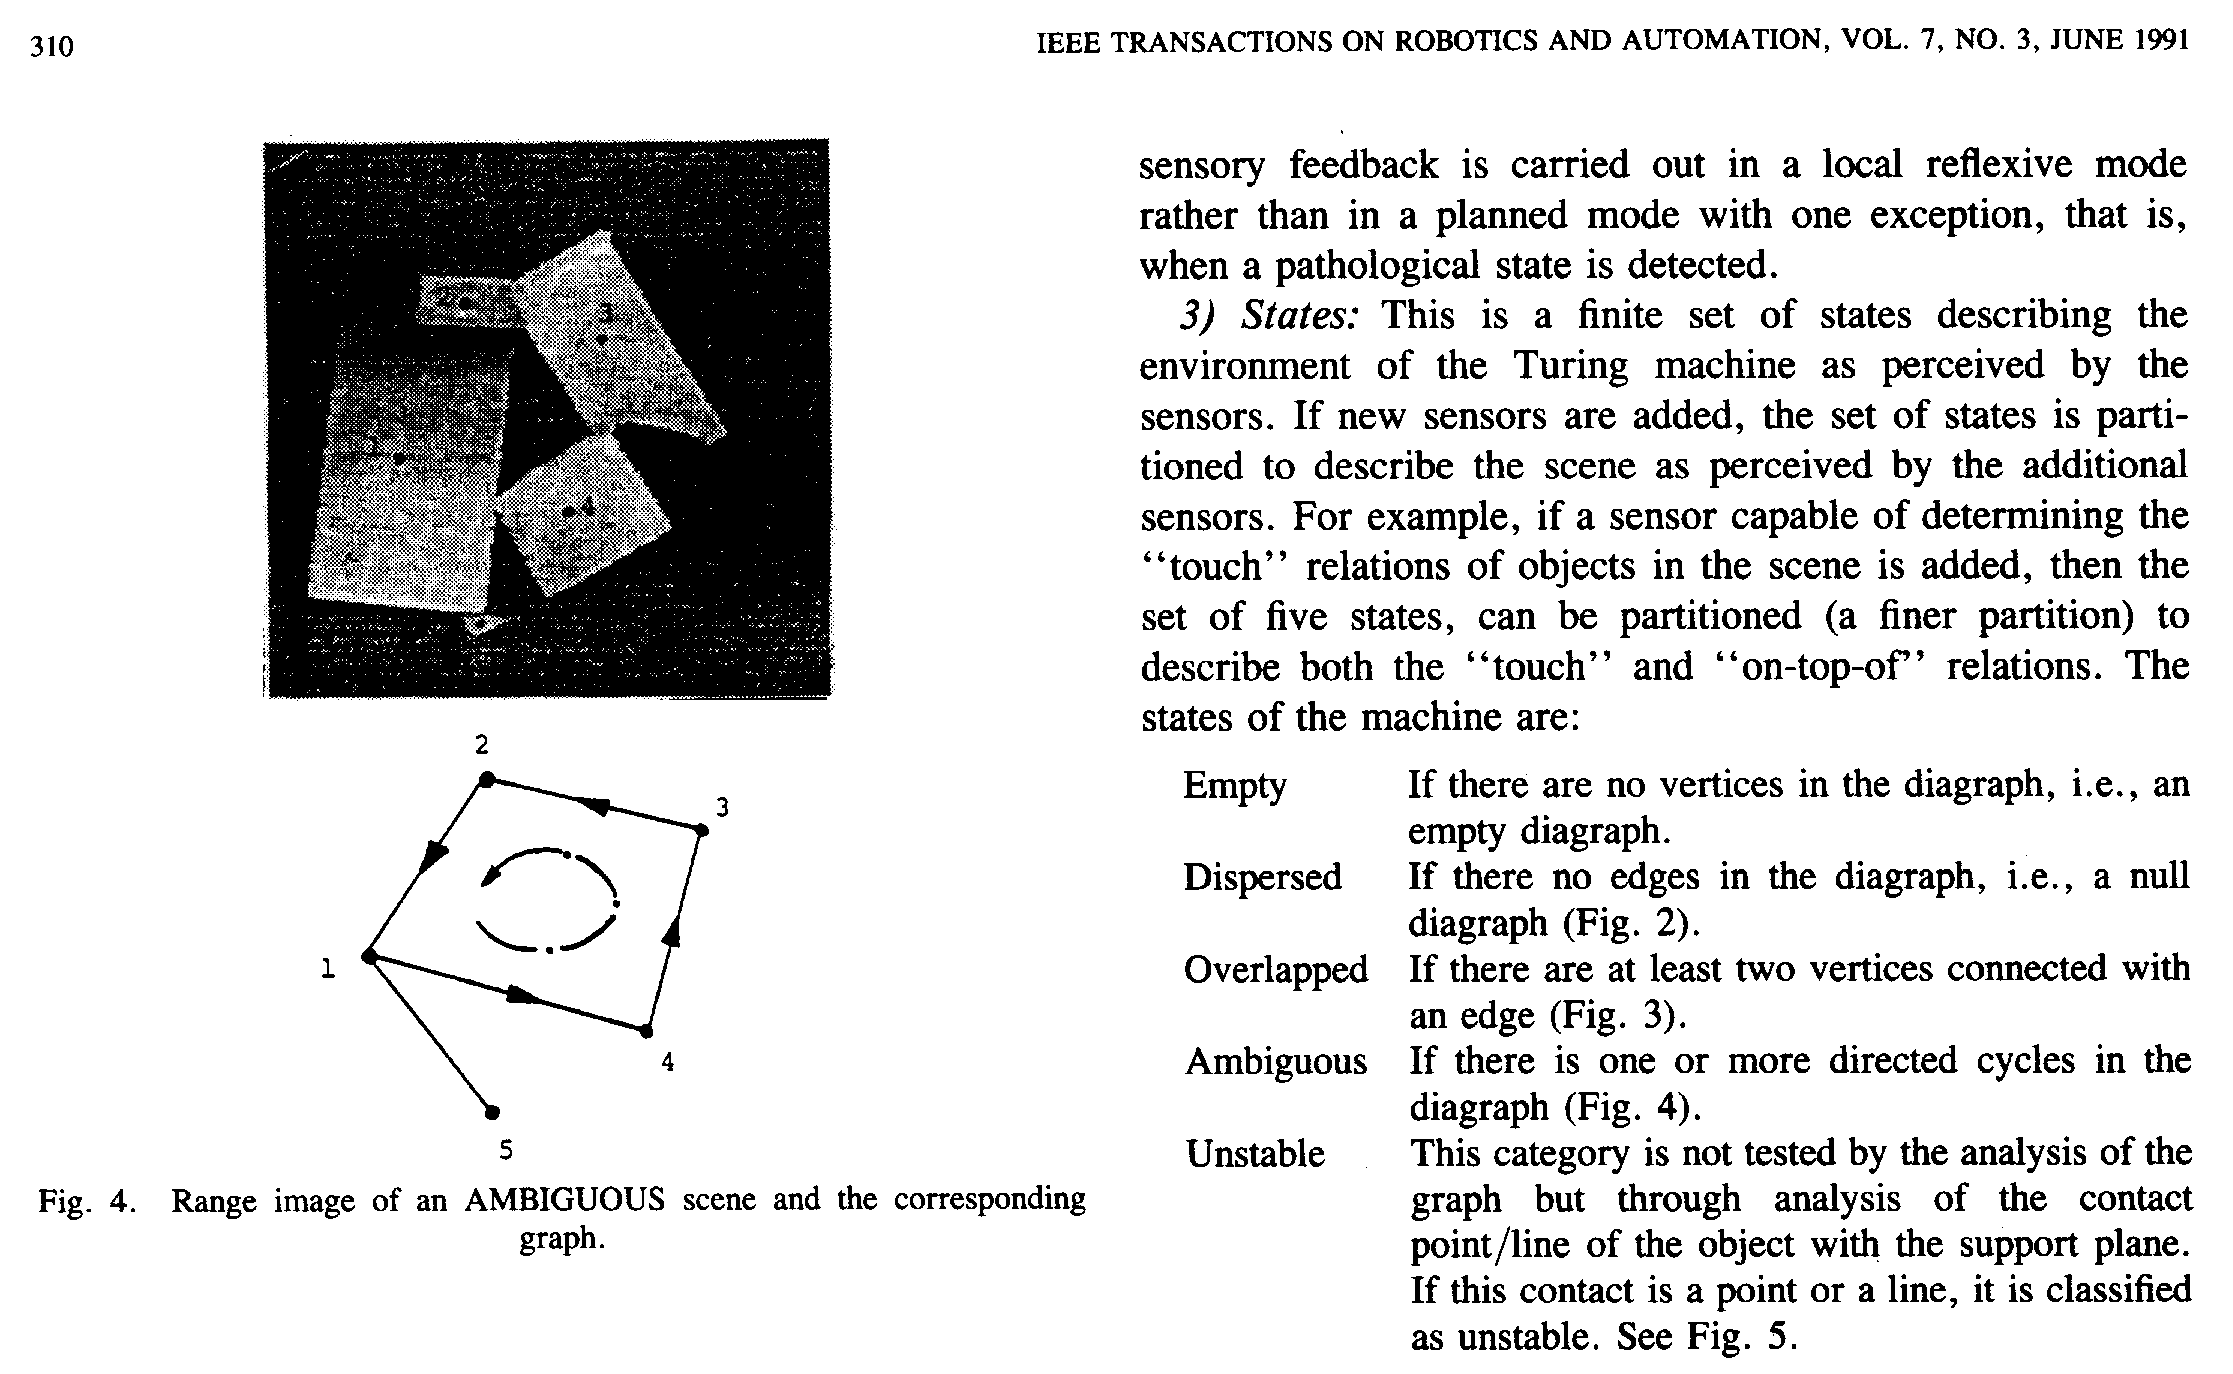
\includegraphics[width=.8\linewidth]{original.png}
  \caption{Imagem original}\label{Fig:original}
\end{figure}


\subsection{O Programa}

O programa foi implementado com Jupyter Notebooks, usando Python 3.7.1. As bibliotecas utilizadas no desenvolvimento do programa foram, com suas respectivas versões: 

\begin{itemize}
    \item numpy (1.15.4): para manipulação dos vetores.

    \item matplotlib (3.0.2): visualização dos dados, resultados finais e intermediários.

    \item opencv (3.4.2): realização da leitura e escrita das imagens, transformação das cores e normalização dos dados. Em especial, deve ser utilizada a versão 3.4.2 pois as anteriores não permitem salvar em formato pbm.
    
    \item scipy (1.1.0): principalmente o pacote \textbf{ndimage} para realizar as diversas operações morfológicas.
\end{itemize}

\subsection{Formato das imagens}

As imagens de entrada estão no formato .pbm. As imagens de saída, tanto as finais quanto as intermediárias também se encontram neste mesmo formato.

\section{Leitura, escrita e plotagem das imagens}

\subsection{Leitura das imagens}

A imagem de entrada é lida com função \textbf{cv2.imread} que armazena a imagem em um \textbf{numpy.ndarray} de 3 dimensões (MxNx3).

Depois de lida, a imagem é convertida para níveis de cinza pela função \textbf{cv2.cvtColor}. Após convertido para escala de cinza, a imagem foi revertida, ou seja, os pixels que estavam descritos como 0 viram 1 e os que estavam como 1 viram 0. Isso se deve ao fato de que, o \textit{openCV} tem como padrão, o branco como sendo 255 e o preto sendo 0. Porém para se aplicar as funções morfológicas, é necessário que o branco (fundo) seja descrito como 0 e o preto, como sendo 1.

\subsection{Escrita das imagens}

Também foi feito uma função auxiliar para facilitar na saída das imagens utilizando a função \textbf{cv2.imwrite}. Porém, assim como foi invertido a imagem quando lida, o mesmo deve ser feito quando escrita depois de aplicar todas as operações morfológicas para o \textit{openCV} conseguir distinguir entre preto e branco novamente.

\subsection{Plotagem das imagens}

Foi utilizado para visualização dos resultados as funções de plotagem de imagens em \textbf{matplotlib.pyplot}, utilizando a paleta de cores em escalas de cinza. Assim como a leitura e escrita, também foi necessário fazer a inversão da imagem antes de plotá-la, uma vez que o \textit{matplotlib} também funciona com o mesmo padrão utilizado pelo \textit{openCV}, onde o 0 representa o preto.

\section{Solução}

\subsection{Componentes conexas}

Para a detecção das componentes conexas na imagem, foram feitas operações morfológicas de dilatação seguida de erosão usando dois diferentes elementos estruturantes: Um contendo 1 pixel de altura e 100 pixels de largura e outro contendo 200 pixels de altura e 1 pixel de largura. As operações foram feitas em duas cópias das imagens originais, de tal forma que uma operação não afetou no desempenho da outra. As seguintes funções foram usadas: \textbf{morphology.binary\_dilatation} e \textbf{morphology.binary\_erosion}

Cada um desses elementos estruturantes foi responsável por agrupar elementos na vertical (no caso do elemento estruturante com 100 pixels de altura) e na horizontal (para o outro elemento estruturante)

Depois de feito as operações nas duas cópias, uma nova imagem foi formada a partir da intersecção dos seus resultados. Foi aplicado em cima desse resultado, a operação de fechamento em um elemento estruturante de 1 de altura e 30 de largura para melhorar as delimitações de cada componente conexa. Foi utilizado a seguinte função (\textbf{morphology.binary\_closing})

Após a operação de fechamento, foi feito uma função auxiliar para identificar cada componente conexa e calcular um retângulo que envolve cada uma delas. Durante a execução dessa função, é verificado se dentro do retângulo definido há de fato algum pixel preto na imagem original ou se a componente conexa foi gerada por ruídos gerados durante as operações morfológicas anteriores. Com isso, foi possível também modificar a imagem colocando um retângulo de 1 pixel de largura envolvendo cada componente conexa descoberta, como demostrado na Figura \ref{Fig:border_components}. Foram obtidas, ao todo, 53 copmponentes conexas.

\begin{figure}[!htb]
    \centering
    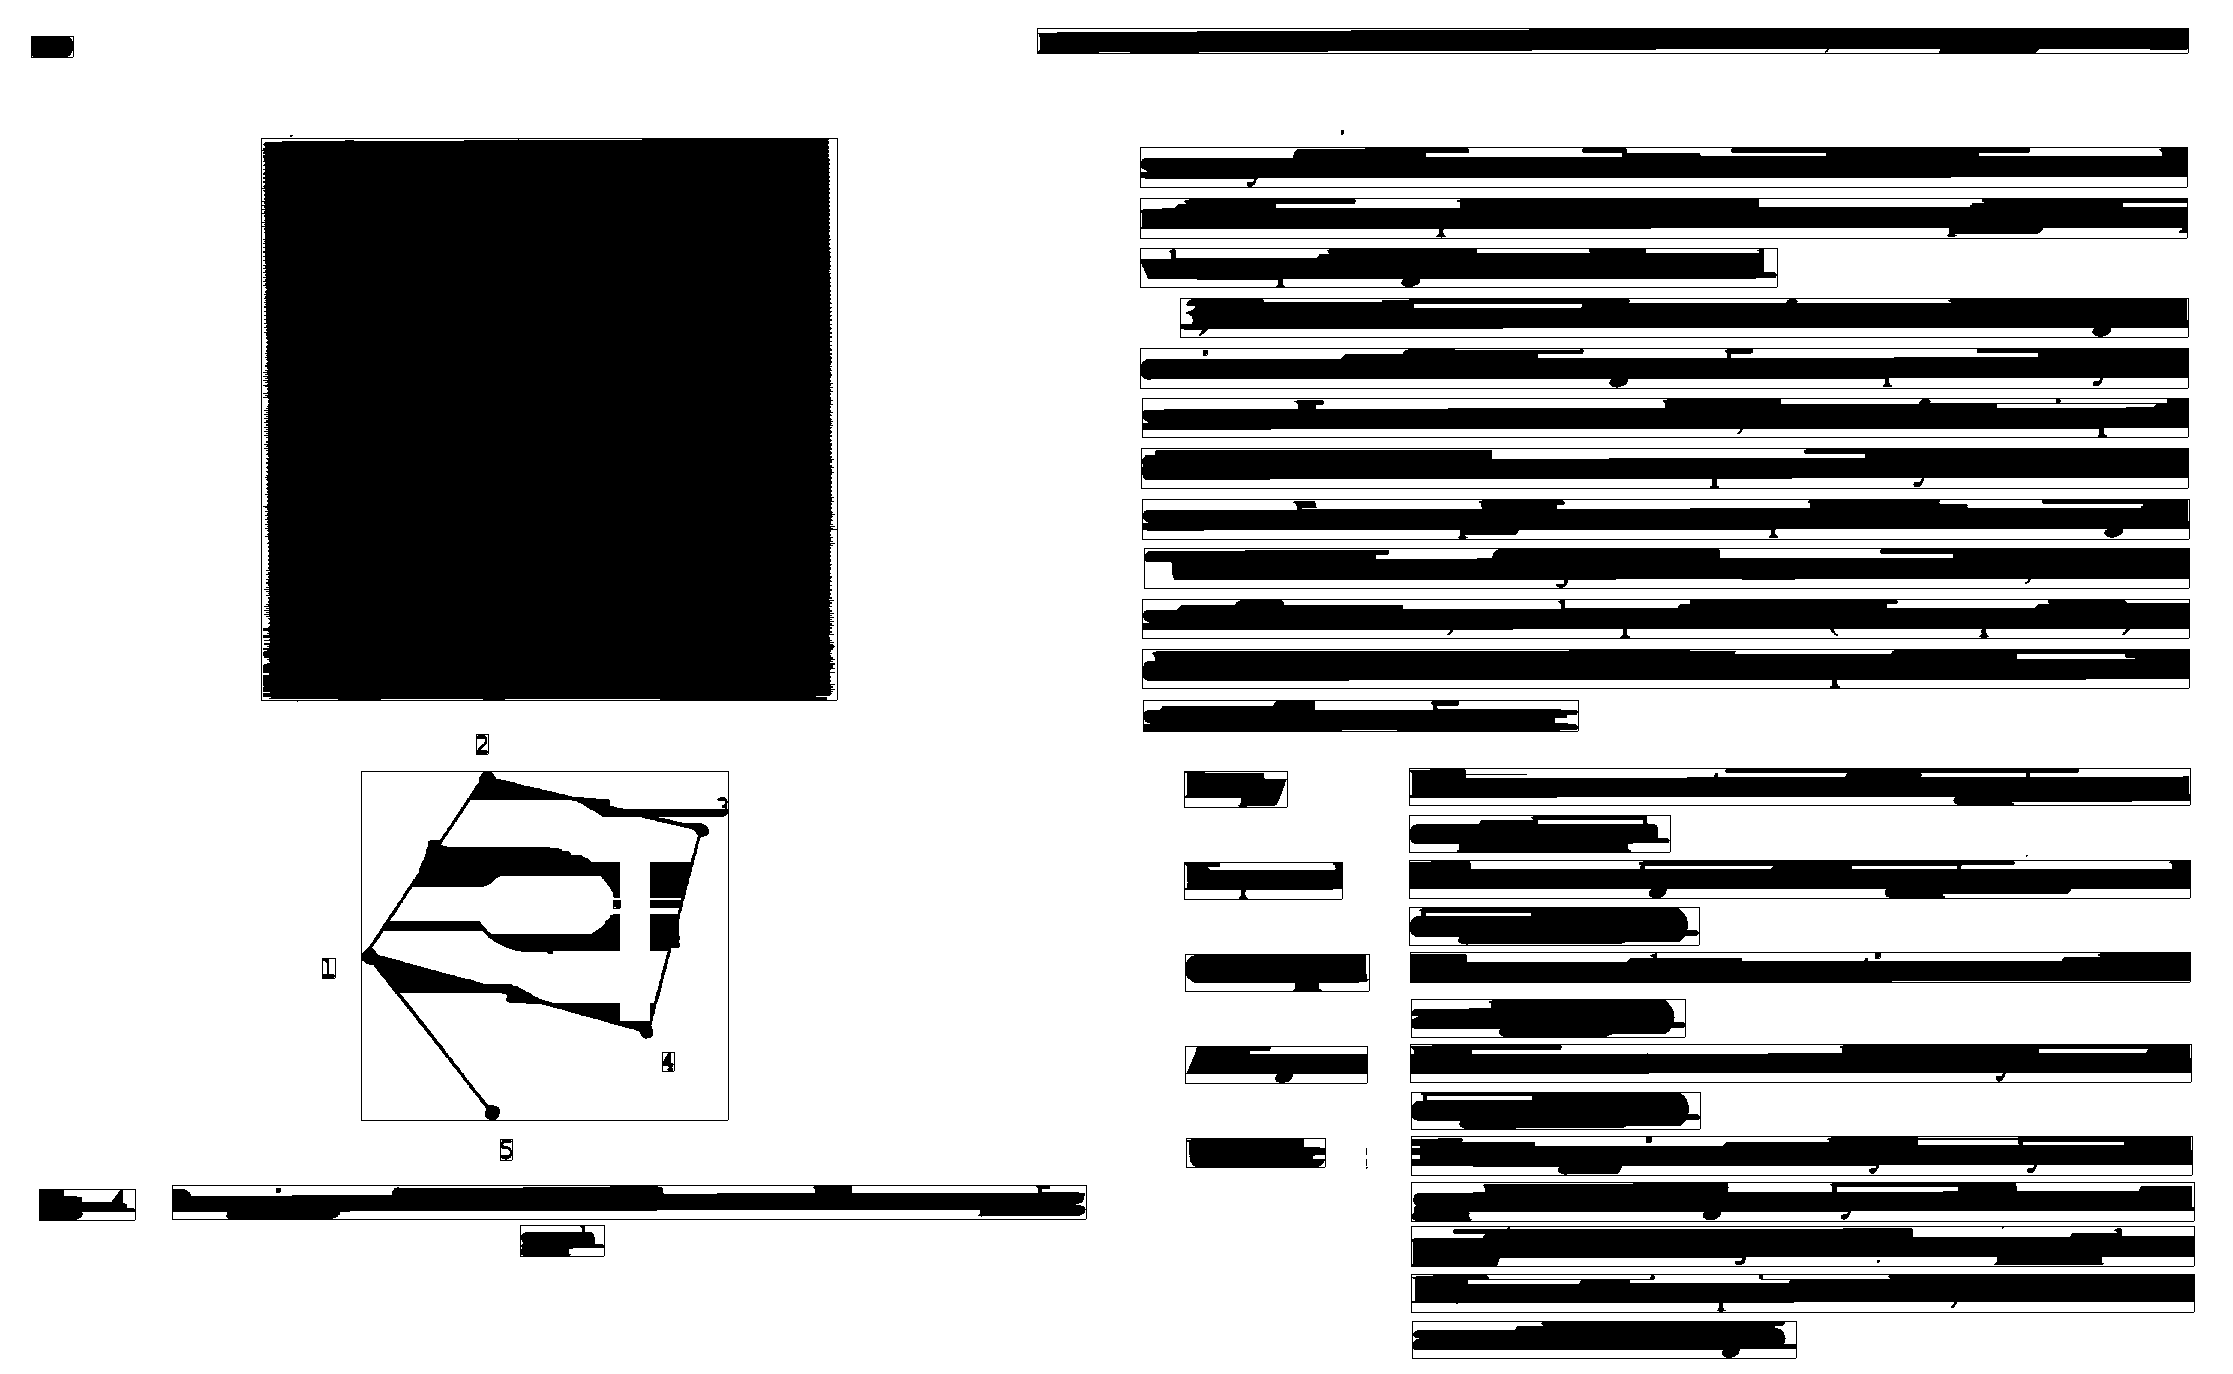
\includegraphics[width=.8\linewidth]{res/bitmap/img_border_components.png}
    \caption{Resultado das operações morfológicas e retângulos definindo cada uma das 53 componentes conexas}\label{Fig:border_components}
\end{figure}

É possível observar que as operações morfológicas acabaram desconsiderando algumas partes das letras como \textit{pingos} nos \textit{is}. Isto se deve porque é feito uma intersecção entre as operações realizadas nas verticais e horizontais. Apesar desses \textit{pingos} estarem presentes utilizando as operações morfológicas com elementos estruturantes de maior altura, alguns desses pingos acabam não sendo capturados pelos elementos estruturantes de maior largura. Dessa maneira, parte desses \textit{pingos} foram considerados como sendo diferentes componentes conexos.

\subsection{Classificação \textit{texto} e \textit{não texto}}

O próximo passo após a detecção das componentes conexas foi suas classificações entre \textit{texto} e \textit{não texto}. Para realizar tal feito, para cada componente conexa descoberta pelo passo anterior, foi realizado o cálculo de duas razões:

\begin{itemize}
  \item razão entre o número de pixel pretos e o número total de pixels (altura x largura);

  \item razão entre o número de transições verticais e horizontais \textit{branco para preto} e o número total de pixels pretos;
\end{itemize}

Para cada uma dessas razões, foi criado uma regra para se classificar os textos entre \textit{texto} e \textit{não texto}. Somente foram consideradas as componentes conexas que possuíam, ao menos, 50 pixels de largura pois dessa forma, evitou-se legendas, numerações de páginas e ruídos. A decisão da proporção usada foi feita apenas por observação dos resultados. 

Seja \textit{b} a razão dos pixels pretos e \textit{i} a razão das inversões chegou-se na seguinte regra:

\[
  X(b,i) = \left\{\begin{array}{lr}
      \text{texto }, &      \text{se } 0.15\leq b\leq 0.60 \text{ e } i > 0.55\\
      \text{não texto }, &  \text{caso contrário }\\
      \end{array}\right\}
\]

Seguindo esta regra, foi detectado um total de 34 linhas contendo textos. Pode-se verificar os resultados na Figura \ref{Fig:border_texts}, onde há retângulos envolvendo cada uma das linhas detectadas.

\begin{figure}[!htb]
  \centering
  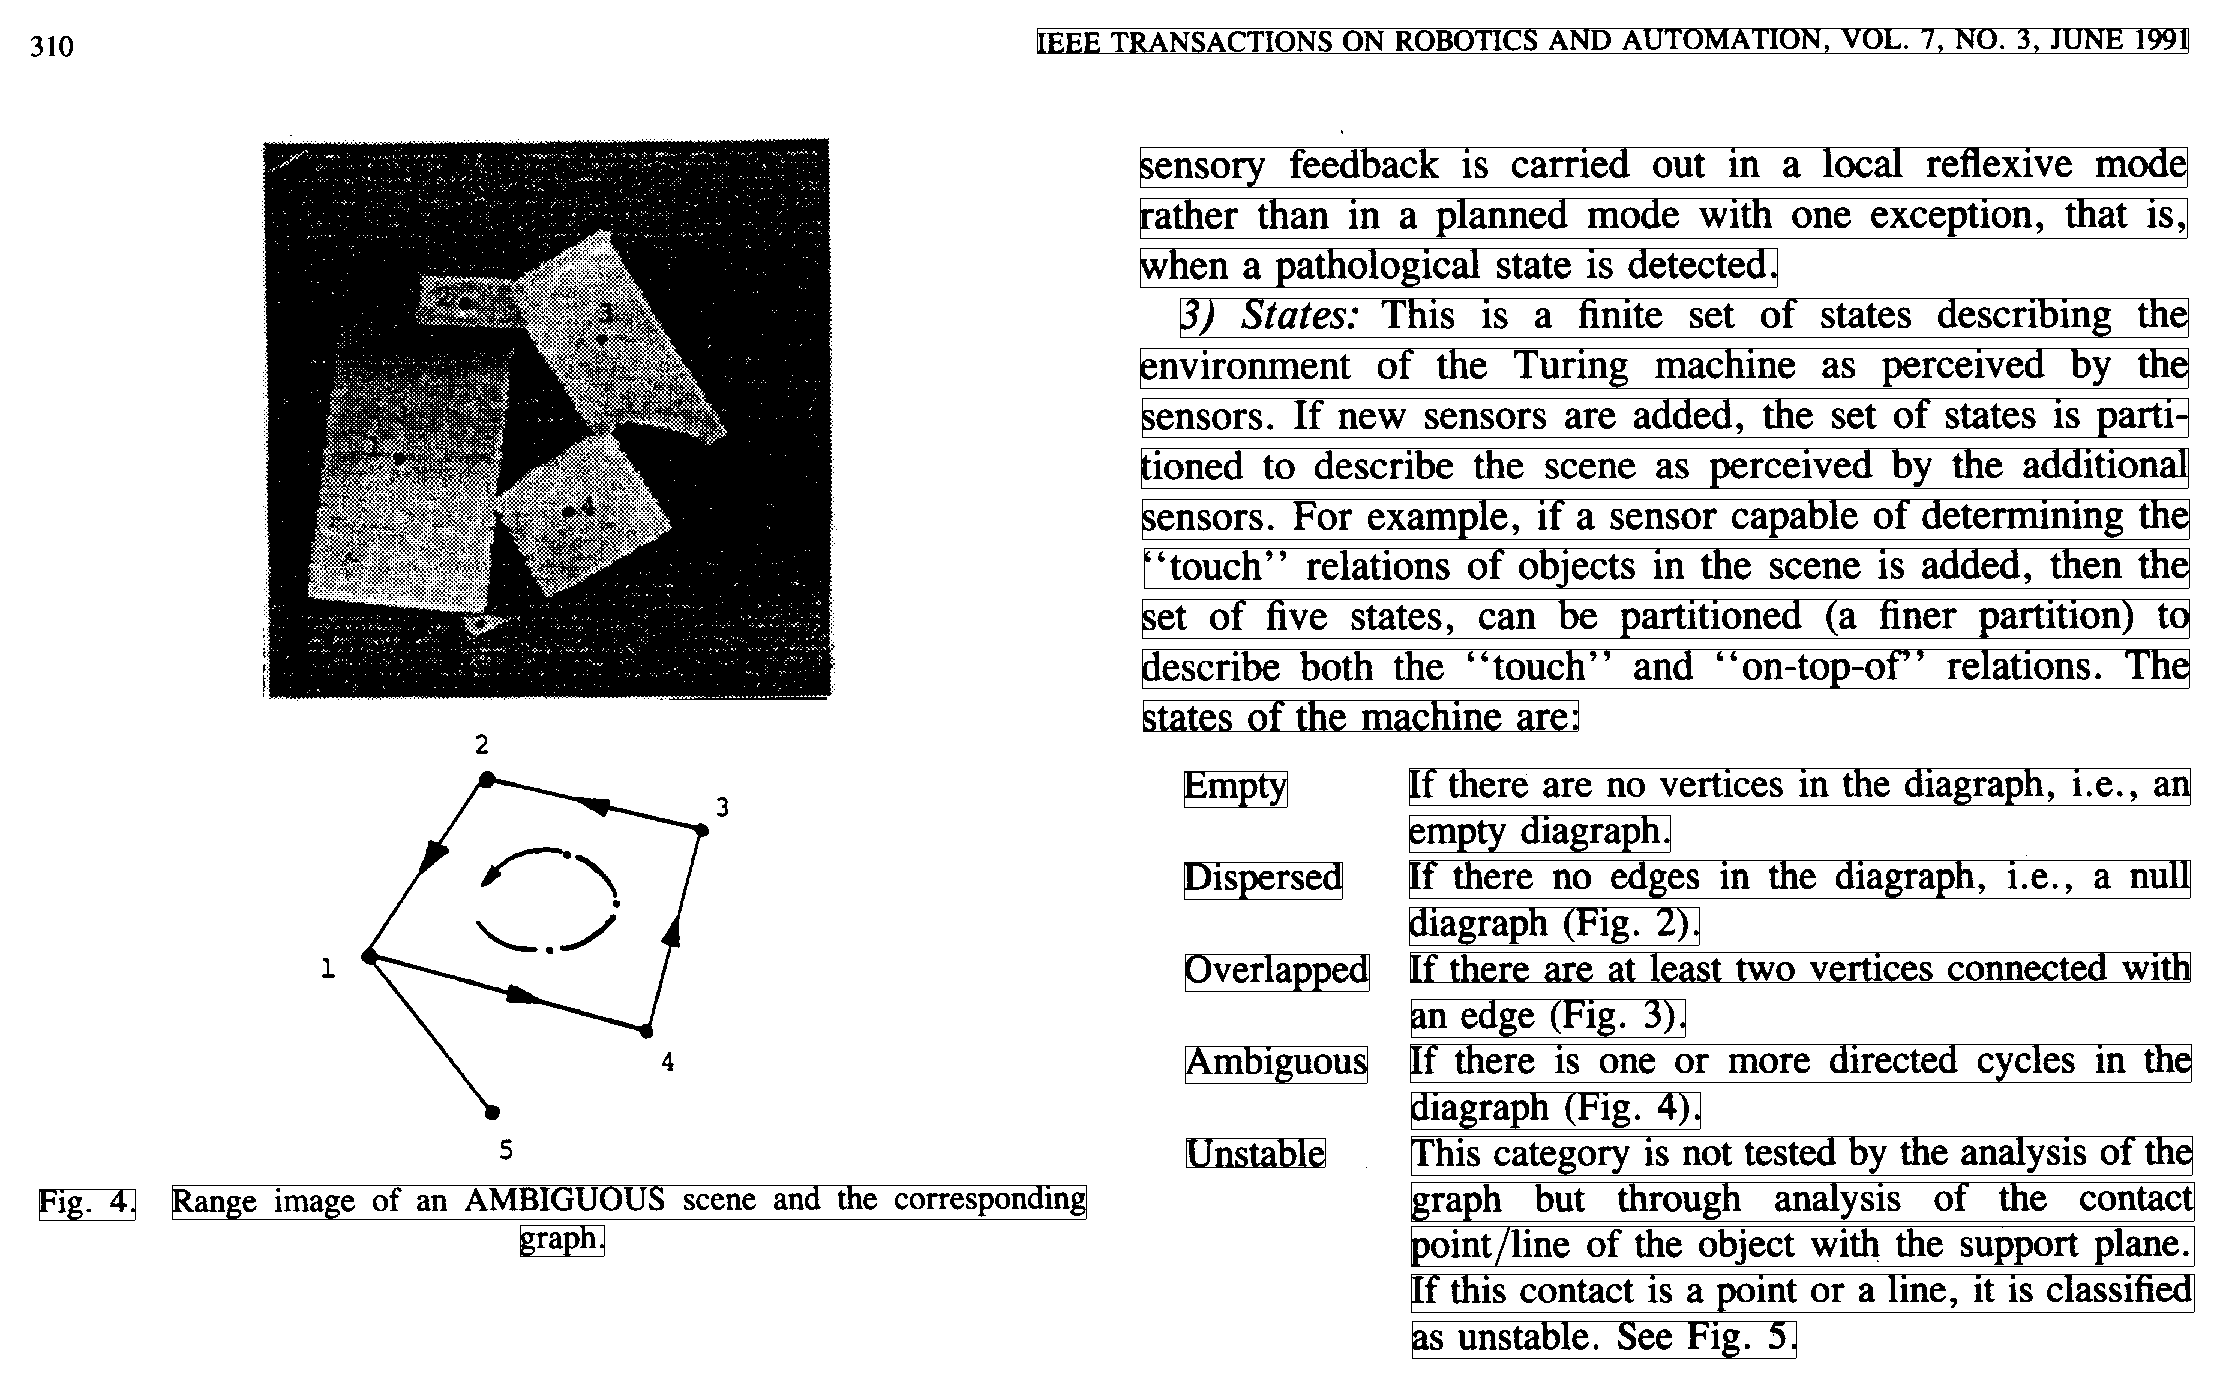
\includegraphics[width=.8\linewidth]{res/bitmap/img_border_texts.png}
  \caption{Resultado das classificação dos textos e retângulos definindo cada uma das 34 linhas classificadas}\label{Fig:border_texts}
\end{figure}

\subsection{Separação das palavras}

Depois de classificado cada uma das componentes conexas em \textit{texto} e \textit{não texto}, deseja-se separar cada palavra de cada linha classificada. Para isso, foi utilizado uma abordagem bem similar a realizada no começo da solução, para detecção das componentes conexas, utilizando operadores morfológicos de fechamento com elementros estruturantes de um certo tamanho para agrupar cada letra de cada palavra. Depois, utilizar a mesma função para obter cada componente conexa (palavra) junto com o retângulo que define cada uma delas.

Para o tamanho do elemento estruturante, foi feito o seguinte cálculo para cada linha descrita na imagem. Pegou-se a altura da imagem e dividiu este valor por 3.5, obtendo um certo fato. Com este fator, foi contruído um elemnto estruturante de altura $ min(30, 3 \cdot fator) $ e largura $ min(30, fator) $. Calculando as dimensões, o algoritmo torna-se mais escalável diante de fontes de tamanhos diferentes onde o espaçamento entre palavras também é diferente.

O tamanho máximo de 30 pixels, foi necessário pois operações de fechamento com elementos estruturantes muito grandes são custosas e causam lentidões durante o processamento. Além disso, a opção por se ter uma altura maior que a largura é justamente para obter \textit{pingos nos is}, pontuações (vírgulas, pontos finais) que antes não eram consideradas.

Aplicando estas operações morfológicasogicas, foi detectado um total de 235 palavras na imagem inteira. Pode-se verificar os resultados na Figura \ref{Fig:border_words}, onde há retângulos envolvendo cada uma das palavras detectadas.

\begin{figure}[!htb]
  \centering
  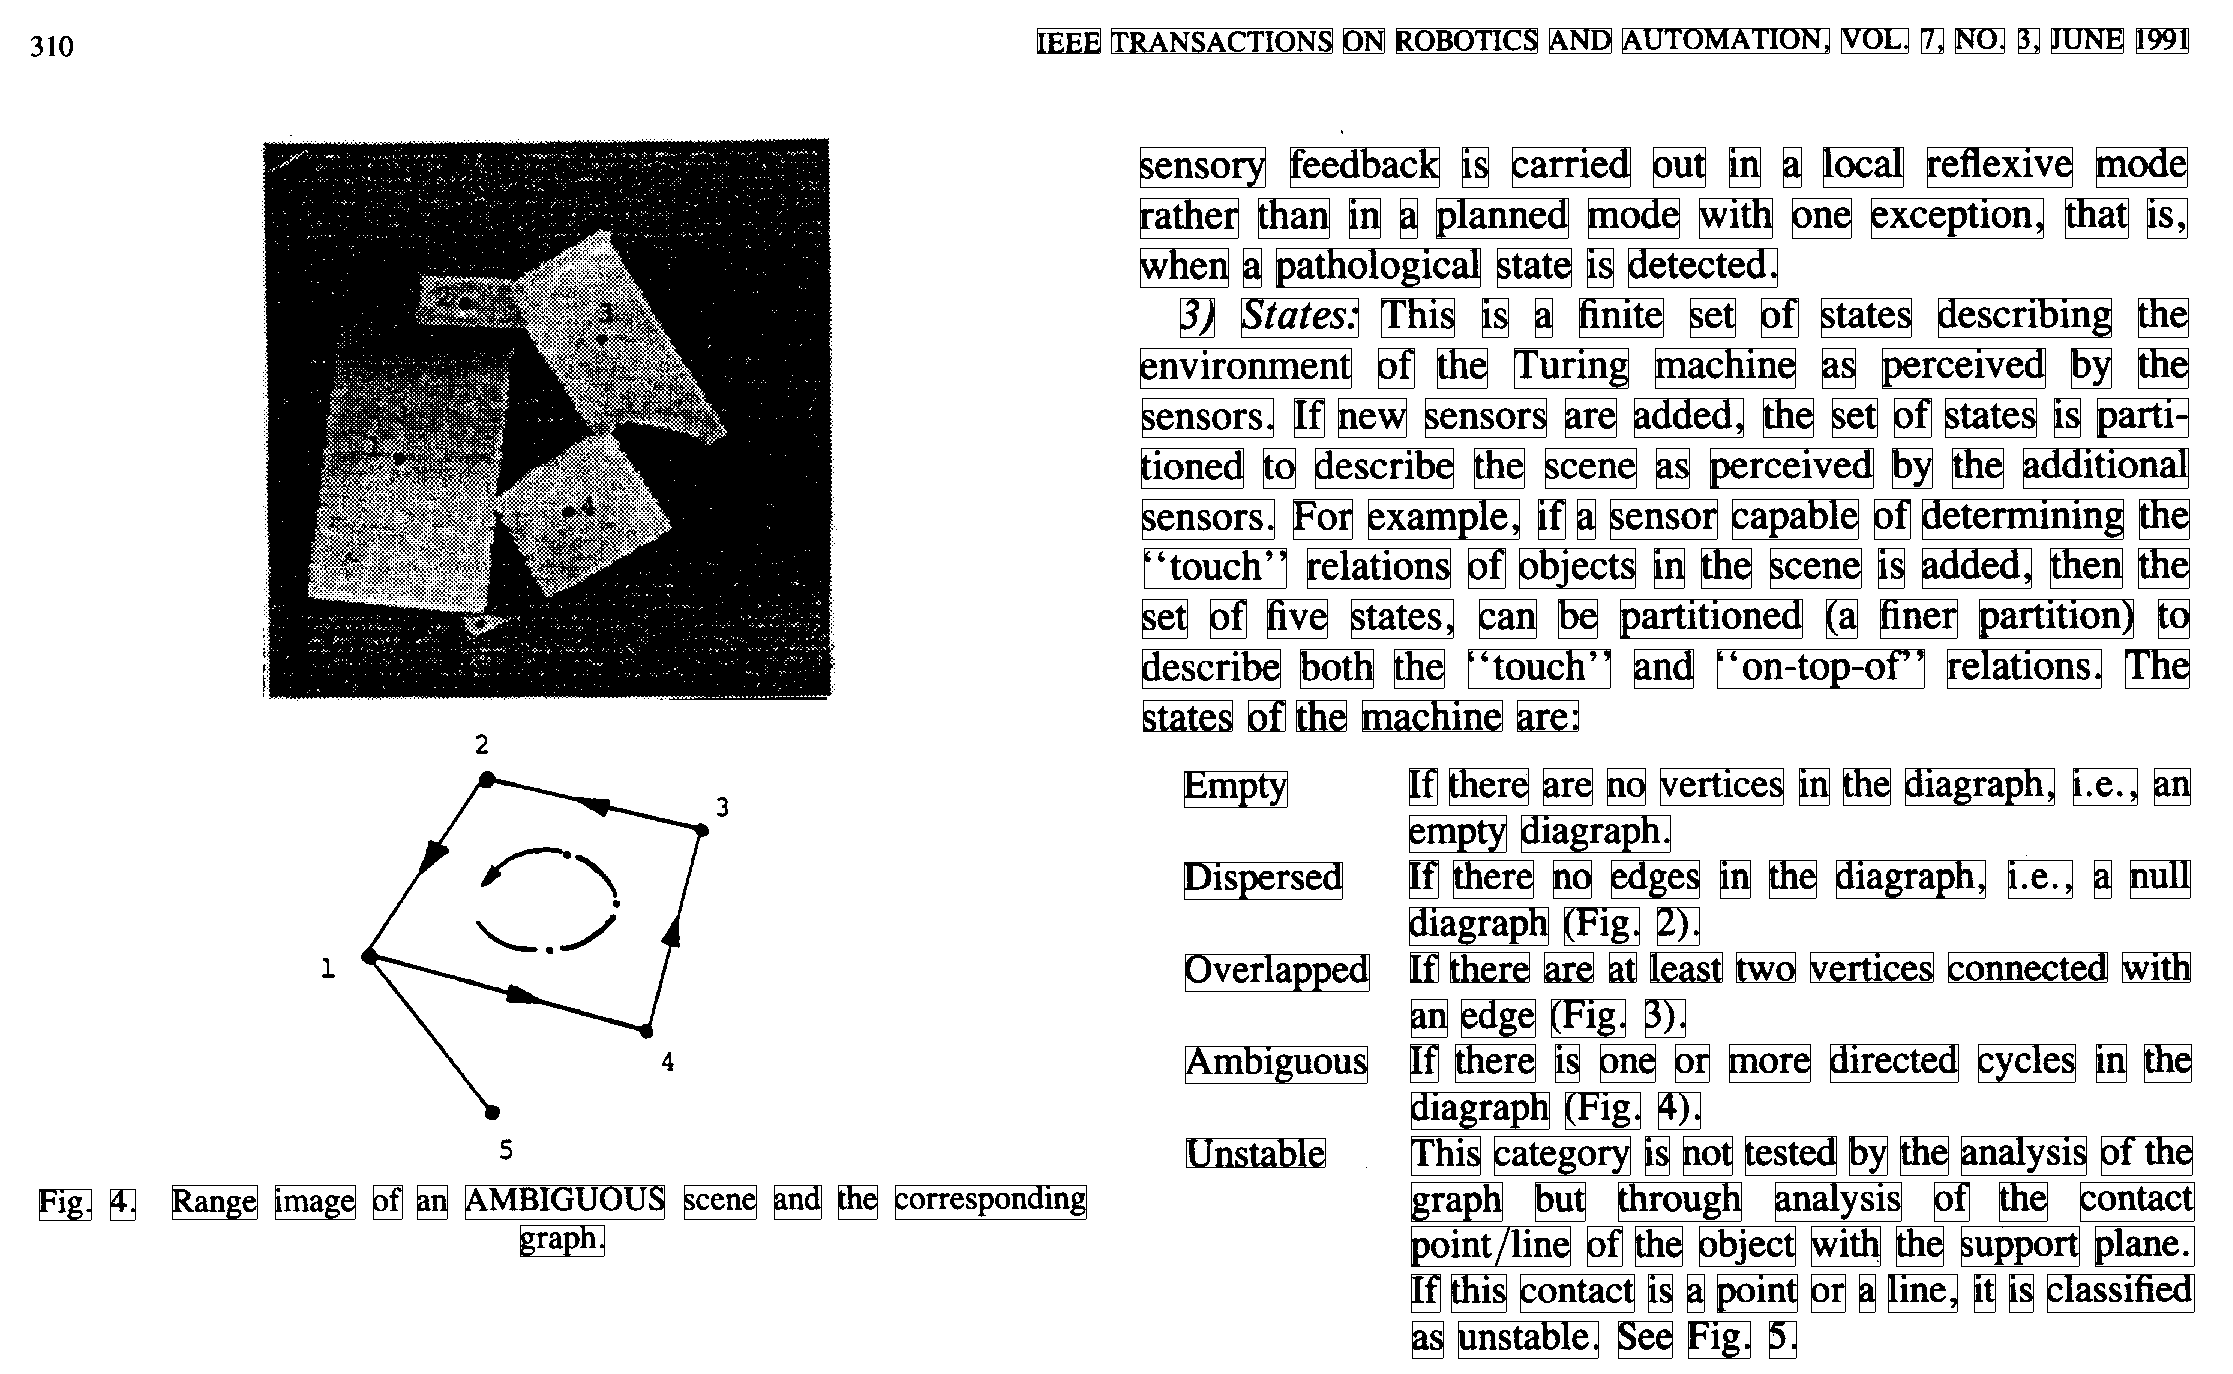
\includegraphics[width=.8\linewidth]{res/bitmap/img_border_words.png}
  \caption{Resultado das classificação dos textos e retângulos definindo cada uma das 34 linhas classificadas}\label{Fig:border_words}
\end{figure}

\section{Conclusão}

Após a execução de todos os procedimentos, pode-se concluir que operadores morfológicos são recursos interessantes para obter componentes conexas para utilizar, por exemplo como feito neste trabalho, classificação de textos.

Porém, há algumas limitações presentes no algoritmo utilizado para a separação das componentes conexas, principalmente quando há elementos que não são textos ao lado de um parágrafo. Tal elemento que não é texto acaba sendo detectado como sendo parte da mesma componente conexa do parágrafo, o que pode gerar resultados questionáveis.

Com a imagem utilizada por padrão neste relatório não foi possível obter este problema. Porém utilizando a imagem \textit{bitmap3.pbm} em anexo juno a este relatório, foi possível reproduzí-lo. Observa-se que a imagem e o texto na imagem \ref{Fig:original3} resultou em uma única componente conexa bem grande pois uniu-se os textos com a imagem ao lado \ref{Fig:erro3}. As linhas abaixo foram detectadas separadamente, formando componentes conexas distintas.

\begin{figure}[!htb]
  \begin{minipage}{0.48\textwidth}
    \centering
    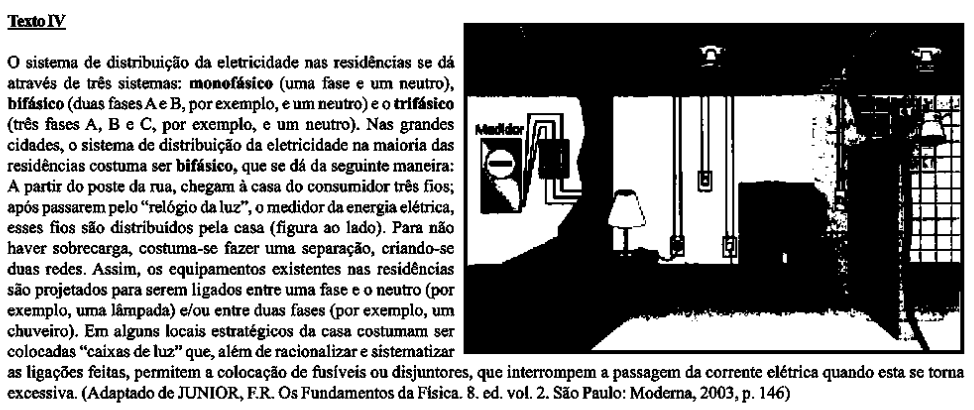
\includegraphics[width=.99\linewidth]{erro2.png}
    \caption{Texto com imagem ao lado}\label{Fig:original3}
  \end{minipage}\hfill
  \begin{minipage}{0.48\textwidth}
    \centering
    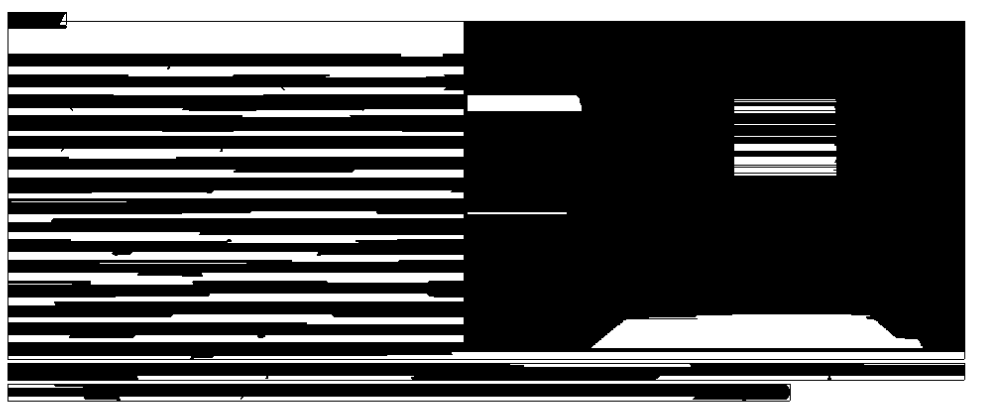
\includegraphics[width=.99\linewidth]{erro1.png}
    \caption{Resultado das componentes conexas após oprações morfológicas}\label{Fig:erro3}
  \end{minipage}
\end{figure}

Além disso, as operações morfológicas junto aos elementos estruturantes escolhidos durante este trabalho se tornaram bem sensíveis a ruídos. Uma possível melhoria do algoritmo seria aplicar filtros para redução de ruídos e elementos indesejáveis antes de se aplicar as operações morfológicas. Porém essas técnincas não foram aplicadas durante o desenvolvimento deste experimento, sendo apenas sugestões para melhorias futuras.

\bibliography{relatorio3}
\bibliographystyle{ieeetr}

\end{document}